\section{Sistema}

\begin{frame}{Sistema de Compressão e Gás Natural}
    \begin{columns}[T] % [T] alinha as colunas pelo topo
        % Coluna da esquerda - Tabela
        \begin{column}{0.48\textwidth}
        \begin{figure}
            \centering
            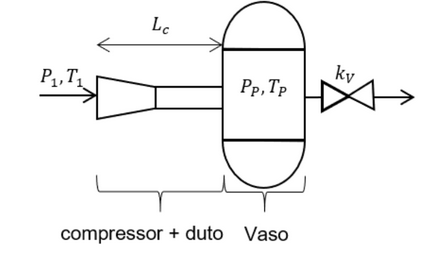
\includegraphics[width=1.1\linewidth]{Figures/compressao.png}
            \caption{Sitema de Compressão retirado de \cite{Meira2022}}
            \label{fig:enter-label}
        \end{figure}
        \end{column}

        % Coluna da direita - Composição e EoS
        \begin{column}{0.52\textwidth}
            \scriptsize
            Composição do gás
                
            O gás natural utilizado é rico em metano, com composição baseada em \cite{Chaczykowski2009}:
            
            \vspace{0.12cm}
            \begin{itemize}  
                \item CH\textsubscript{4}: 98,34\% \quad C\textsubscript{2}H\textsubscript{6}: 0,61\%
                \item C\textsubscript{3}H\textsubscript{8}: 0,15\% \quad iC\textsubscript{4}H\textsubscript{10}: 0,03\%
                \item nC\textsubscript{4}H\textsubscript{10}: 0,03\% \quad CO\textsubscript{2}: 0,80\%
                \item Traços de: iC\textsubscript{5}H\textsubscript{12}, nC\textsubscript{5}H\textsubscript{12}, N\textsubscript{2}
            \end{itemize}
            \vspace{0.1cm}
            A equação de estado de \cite{Soave1972} foi utilizada para modelar o comportamento termodinâmico do gás:

            \[
            P = \frac{R T}{V - b} - \frac{a(T)}{V(V + b)}
            \]

            com:
            \begin{itemize}
                \item \( a(T) \): fator de correção das forças intermoleculares
                \item \( b \): correção do volume molecular
            \end{itemize}
        \end{column}
    \end{columns}
\end{frame}



\begin{frame}{Equações e Variáveis do Modelo de \cite{Meira2022} }
    \scriptsize
    \textbf{Equações diferenciais que descrevem a dinâmica do sistema:}

    \begin{multicols}{2}
    % Coluna da esquerda: equações diferenciais
    \begin{align}
        \frac{d\dot{m}}{dt} &= \frac{A_1}{L_c}(P_2 - P_P) \tag{1} \\
        \frac{dV_P}{dt} &= -\frac{V_P^2}{v_{PM}} \left( \dot{m} - \alpha k_v \sqrt{P_P - P_{\text{out}}} \right) \tag{2} \\
        \frac{dT_P}{dt} &= 
        \begin{aligned}[t]
            &\frac{V_P \dot{m}}{v_P M} \left( \frac{h_c - h_p}{C_V} \right) + \\
            + &\frac{R_a T_P}{C_V} \left[ T_P \left( \frac{\partial Z_P}{\partial T} \right)_{V_P} + Z_P \right]
            \frac{V_P}{v_P M} \left( \dot{m} - \alpha k_v \sqrt{P_P - P_{\text{out}}} \right)
        \end{aligned} \tag{3} \\
        \textbf{f(u, x, z)} &= 0 \tag{4}
    \end{align}

    \columnbreak
    % Coluna da direita: variáveis algébricas
    \begin{minipage}{\linewidth}
        \textbf{Variáveis algébricas estimadas:}
        \begin{itemize}
            \item \( P_2 \), \( T_2 \), \( V_2 \): saída do compressor
            \item \( T_{2s} \), \( V_{2s} \): pós-compressão isentrópica
            \item \( V_1 \): sucção do compressor
            \item \( V_{imp} \), \( T_{imp} \): impelidor
            \item \( V_{dif} \), \( T_{dif} \): difusor
            \item \( P_P \): pressão no plenum
        \end{itemize}
    \end{minipage}
    \end{multicols}
\end{frame}